\chapter[Zásuvný modul]{Zásuvný modul 
\includegraphics[scale=0.65]{./pictures/ikonka.png}\footnote{Tady ocitovat ikonku, že je od kolegy ze SÚRA}}
\label{4-plugin}

V následujícím textu bude popsán postup tvorby nového softwarového nástroje \textit{Ground radiation monitoring} a jeho funkcionalita. Při vývoji nástroje bylo čerpáno z doporučené literatury SEM DÁT TY KNÍŽKY ZE ZADÁNÍ. 

\section{Zadání}
Zadáním bakalářské práce bylo vytvoření softwarového nástroje, který ze vstupní interpolované mapy dávkových příkonů extrahuje data do naplánovaných tras monitorování a vypočítá obdrženou dávku záření gama při zadané rychlosti. Nástroj dále vypočte jednoduché statistiky, maximální a průměrný dávkový příkon, délku trasy, čas a~kumulativní dávku v~určitých zadaných intervalech.

\subsection{Vstupní data}
\begin{enumerate}
	\item \textbf{Interpolovaná mapa dávkového příkonu} \\
	Je vytvořena v rastrovém formátu, který je podporován knihovnou GDAL. Obsahuje hodnoty dávkového příkonu v daných jednotkách. (Plugin umožňuje volit typ jednotek). Mapa je v souřadnicovém systému WGS84 EPSG:4326.
	\item \textbf{Trasa monitorování} \\
	Je vytvořena ve vektorovém formátu, který je podporován knihovnou OGR. Trasy mohou být generované pomocí plánovačů tras, např. společnosti Google, Inc. Trasa monitorování je taktéž v souřadnicovém systému WGS84 EPSG:4326. 
\end{enumerate}

			\begin{figure}[H]
    			\centering
      			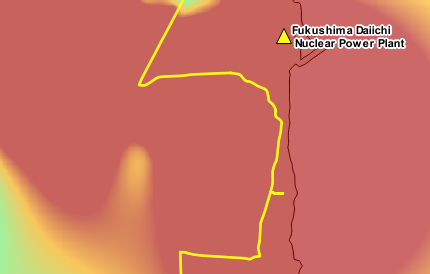
\includegraphics[scale=0.7]{./pictures/ukazka_vstupnich_dat.png}
      				\caption[Ukázka vstupních dat]{Ukázka vstupních dat}(zdroj: co sem napsat?)
     				\label{fig:vstup}
  			\end{figure}
  			
\subsection{Výstupní data}
\begin{enumerate}
	\item \textbf{Soubor se zprávou o výpočtu} \\
	Soubor se zprávou o výpočtu v textovém formátu (\textit{.txt}) obsahuje následující informace o výpočtu (v anglickém jazyce):
		\begin{itemize}
			\item čas vytvoření zprávy (\textit{report created})
			
			\item informace o trase (\textit{route information})
			\begin{itemize}
				\item název trasy (\textit{route})
				\item zadaná rychlost v km/h (\textit{monitoring speed (km/h)})
				\item celkový čas monitorování v h:mm:ss (\textit{total monitoring time (h:mm:ss)})
				\item celková vzdálenost v km (\textit{total distance (km)})
			\end{itemize}
			
			\item informace o části trasy bez dostupných dat (v místech, kde trasa přesahuje mapu dávkového příkonu) (\textit{no data})
			\begin{itemize}
				\item čas (\textit{time})
				\item vzdálenost v km (\textit{distance (km)})
			\end{itemize}
			
			\item statistické hodnoty (\textit{radiation values (estimated)})
			\begin{itemize}
				\item maximální dávkový příkon v $\mu$Sv/h (\textit{maximum dose rate ($\mu$Sv/h)})
				\item průměrný dávkový příkon v $\mu$Sv/h (\textit{average dose rate ($\mu$Sv/h)})
				\item celková dávka v $\mu$Sv (\textit{total dose ($\mu$Sv)})
			\end{itemize}
			
			\item nastavení (\textit{plugin settings})
			\begin{itemize}
				\item jednotky dávkového příkonu vstupní mapy (\textit{input raster units})
				\item vzdálenost mezi body navzorkované trasy v m (vysvětleno v kapitole NAPSAT KDE JE VYSVĚTLENÝ VZORKOVÁNÍ (\textit{distance between track vertices (m)})
			\end{itemize}
			
		\end{itemize}
	
			\begin{figure}[H]
    			\centering
      			
\includegraphics[scale=0.8]{./pictures/report.png}
      				\caption[Ukázka zprávy o výpočtu]{Ukázka zprávy o výpočtu}(zdroj: co sem napsat?)
     				\label{fig:report}
  			\end{figure}
  			
	\item \textbf{Soubor trasy} \\
	Soubor trasy obsahuje bodovou vrstvu ve formátu Esri Shapefile (\textit{.shp}) s body trasy navzorkované dle zadání uživatele (bude vysvětleno v kapitole NAPSAT KDE JE VYSVĚTLENÝ VZORKOVÁNÍ) s následujícími atributy:
		\begin{itemize}
			\item dávkový příkon
			\item kumulativní čas
			\item časový interval mezi body
			\item kumulativní dávka
		\end{itemize}
			\begin{figure}[H]
    			\centering
      			
\includegraphics[scale=0.8]{./pictures/atributova_tabulka.png}
      				\caption[Výřez atributové tabulky]{Výřez atributové tabulky}(zdroj: co sem napsat?)
     				\label{fig:atributova_tabulka}
  			\end{figure}
  	
  	\item \textbf{Soubor s údaji o trase (volitelné)} \\
  	V souboru s údaji o trase ve formátu CSV (\textit{.csv}, hodnoty oddělené čárkou) jsou obsaženy stejné hodnoty jako v atributové tabulce navzorkované trasy. Navíc soubor obsahuje souřadnice bodů. Vytvoření souboru je volitelné. 
  			\begin{figure}[H]
    			\centering
      			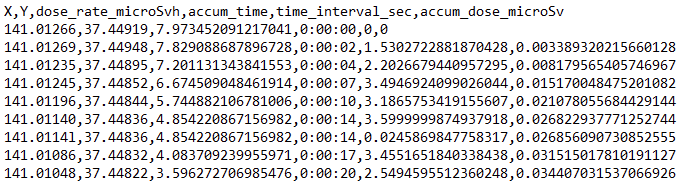
\includegraphics[scale=0.8]{./pictures/csv.png}
      				\caption[Výřez ze souboru s hodnotami oddělenými čárkou]{Výřez ze souboru s hodnotami oddělenými čárkou}(zdroj: co sem napsat?)
     				\label{fig:csv}
  			\end{figure}	
\end{enumerate}

\section{Popis kódu(pracovní název)}
\subsection[Plugin Builder]{Plugin Builder 
\includegraphics[scale=0.1]{./pictures/plugin_builder.png}}
K vytvoření základu softwarového nástroje byl použit zásuvný modul Plugin Builder dostupný z oficiálního QGIS repozitáře.\footnote{Dostupné z \url{https://plugins.qgis.org/plugins/pluginbuilder/}} Tento modul pochází z dílny organizace GeoApt LLC, jež se zabývá volně šiřitelným GIS. Po zadání základních informací (název modulu, základní popis, autor, požadovaná verze QGIS, odkazy a další údaje o repozitáři apod.) Plugin Builder vytvoří kostru nového zásuvného modulu. Tato kostra zajišťuje jeho základní funkcionalitu, tedy zobrazení okna a jeho vypnutí, potažmo tlačítka \texttt{OK | Cancel}, pokud není nastaveno, že okno zásuvného modulu bude "přichycovací". 

\subsection{Popis souborů}
Celý zásuvný modul \textit{Ground radiation monitoring} tvoří několik souborů dohromady tvořících balíček, který zajišťuje spustitelnost a funkcionalitu modulu. Některé soubory zde budou prezentovány. Funkcionalita zásuvného modulu zajišťující řešení zadání bakalářské práce je uložena v posledních dvou jmenovaných souborech, které obsahují modifikace a bloky kódu zaručující výsledky práce. %tohle napsat nějak lépe kámo

\begin{itemize} %to mam z Mastering QGIS, ještě že mastruju
	\item \textbf{\_\_init\_\_.py} \\ 
		Tento soubor slouží pro základní inicializaci modulu.
		 
	\item \textbf{metadata.txt} \\
		Tento textový soubor obsahuje informace o zásuvném modulu čtené Správcem zásuvných modulů. Vedle údajů jako je jméno autora a název modulu je zde například také údaj o požadované verzi QGIS, pro kterou je modul naprogramován. Správce pak tento údaj porovná s verzí QGIS a pokud dojde ke konffliktu, tak vypíše chybovou hlášku a modul nenaimportuje.
	
	\item \textbf{Makefile} \\
		V tomto souboru se nachází set instrukcí např. pro zkompilování dokumentace nebo souboru \textbf{resources.qrc} (zkompilovaná verze je \textbf{resources.py}), který informuje Qt jak naložit s ikonou modulu.
		
	\item \textbf{plugin\_upload.py} \\
		Tento soubor pro nahrání modulu do QGIS repozitáe zásuvných modulů.

	\item \textbf{ground\_radiation\_monitoring.py} \\
		Tento soubor slouží pro implementaci zásuvného modulu do prostředí QGIS. Obsahuje třídu \texttt{GroundRadiationMonitoring}, jejíž zásadními metodami jsou \texttt{add\_action} - metoda načítající ikonu modulu (včetně názvu) do nástrojové lišty QGIS a do menu, tedy přidává tlačítko na spuštění. Dále jsou to metody \texttt{onClosePlugin} a \texttt{unload}, které se starají o destrukci modulu.

	\item \textbf{ground\_radiation\_monitoring\_dockwidget.py} \\
		Tento soubor zajišťuje propojení s grafickým rozhraním, které je vytvořené v souboru \textbf{ground\_radiation\_monitoring\_base.ui} pomocí prostředí QT Designer. Obsahuje třídu \texttt{GroundRadiationDockWidget}, ve které jsou implementovány metody pro načítání vstupních dat, čtení údajů zadaných uživatelem, především také pro spuštění (a případné přerušení) procesu výpočtu a práci s výstupním souborem trasy (pokud si to uživatel přeje, vrstva s trasou může být načtena do QGIS). V případě chyby při zadání vstupních parametrů (např. zadání textu do pole, do kterého má být zadané číslo nebo výběr výstupního souboru, do kterého je zákaz zápisu) je uživatel upozorněn chybovým hlášením.     
	
	\item \textbf{ground\_radiation\_monitoring\_computation.py} \\
		V tomto souboru probíhá samotný výpočet dle uživatelsky zadaných dat a vstupních parametrů. Obsahuje třídu \texttt{GroundRadiationMonitoringComputation}, která je implementována jako samostatné výpočetní vlákno. Toto má za výhodu, že výpočet probíhá na pozadí, tedy že s QGIS se dá pracovat dále nezávisle na probíhajícím procesu, což je nezbytné vzhledem k jeho někdy dlouhému trvání (v závislosti na vstupních proměnných). V této třídě jsou vedle výpočetních metod také metody pro vytváření výstupních souborů. Třída během výpočtu komunikuje s hlavním vláknem (s třídou \texttt{GroundRadiationMonitoringDockWidget}) přes signály, pomocí kterých informuje o postupu výpočtu, který je zobrazován v ukazateli průběhu výpočtu.
	
\end{itemize}

\subsection{Vzorkování linie}


\section{Testování}
Popsat testovací data (použily se tyhle, k tomu obrázky).

